% Author: Nelson Lago
% This file is distributed under the MIT Licence

%%%%%%%%%%%%%%%%%%%%%%%%%%%%%%%%%%%%%%%%%%%%%%%%%%%%%%%%%%%%%%%%%%%%%%%%%%%%%%%%
%%%%%%%%%%%%%%%%%%%%%%%%%%%%%%%%% PREÂMBULO %%%%%%%%%%%%%%%%%%%%%%%%%%%%%%%%%%%%
%%%%%%%%%%%%%%%%%%%%%%%%%%%%%%%%%%%%%%%%%%%%%%%%%%%%%%%%%%%%%%%%%%%%%%%%%%%%%%%%

% A língua padrão é a última da lista
\documentclass[a1paper,brazilian,english]{article}

% Vários pacotes e opções de configuração genéricos
\usepackage{imegoodies}
\usepackage[poster,hidelinks]{imelooks}
% \tcbposterset{fontsize = 32pt} % default, mude se necessário
\usepackage{graphicx} % For including images
\usepackage{caption}  % For the \captionof command

% Diretórios onde estão as figuras; com isso, não é necessário (mas
% é permitido) colocar o caminho completo em \includegraphics. Note
% que a extensão nunca é necessária (mas é permitida), ou seja, o
% resultado é o mesmo com "\includegraphics{figuras/foto.jpeg}",
% "\includegraphics{foto.jpeg}", "\includegraphics{figuras/foto}"
% ou "\includegraphics{foto}".
\graphicspath{{figuras/},{fig/},{logos/},{img/},{images/},{imagens/}}

% Comandos rápidos para mudar de língua:
% \en -> muda para o inglês
% \br -> muda para o português
% \texten{blah} -> o texto "blah" é em inglês
% \textbr{blah} -> o texto "blah" é em português
\babeltags{br = brazilian, en = english}


%%%%%%%%%%%%%%%%%%%%%%%%%%%%%%%%%%%%%%%%%%%%%%%%%%%%%%%%%%%%%%%%%%%%%%%%%%%%%%%%
%%%%%%%%%%%%%%%%%%%%%%%%%%%%%%%%%% METADADOS %%%%%%%%%%%%%%%%%%%%%%%%%%%%%%%%%%%
%%%%%%%%%%%%%%%%%%%%%%%%%%%%%%%%%%%%%%%%%%%%%%%%%%%%%%%%%%%%%%%%%%%%%%%%%%%%%%%%

% O arquivo com os dados bibliográficos para biblatex; você pode usar
% este comando mais de uma vez para acrescentar múltiplos arquivos
\addbibresource{bibliografia.bib}

% Este comando permite acrescentar itens à lista de referências sem incluir
% uma referência de fato no texto (pode ser usado em qualquer lugar do texto)
%\nocite{bronevetsky02,schmidt03:MSc, FSF:GNU-GPL, CORBA:spec, MenaChalco08}
% Com este comando, todos os itens do arquivo .bib são incluídos na lista
% de referências
%\nocite{*}


%%%%%%%%%%%%%%%%%%%%%%%%%%%%%%%%%%%%%%%%%%%%%%%%%%%%%%%%%%%%%%%%%%%%%%%%%%%%%%%%
%%%%%%%%%%%%%%%%%%%%%%%%%%%%%%% INÍCIO DO POSTER %%%%%%%%%%%%%%%%%%%%%%%%%%%%%%%
%%%%%%%%%%%%%%%%%%%%%%%%%%%%%%%%%%%%%%%%%%%%%%%%%%%%%%%%%%%%%%%%%%%%%%%%%%%%%%%%


% Existem várias packages para criar pôsteres com LaTeX (a0poster, baposter,
% tikzposter, sciposter...). As mais comuns atualmente são beamerposter
% e tcolorbox (com sua biblioteca "poster"). Ambas funcionam muito bem;
% beamerposter é mais familiar (ela simplesmente utiliza beamer com alguns
% ajustes no tamanho das fontes e do papel), mas com tcolorbox o alinhamento
% vertical dos elementos é MUITO mais simples, e esta é a solução adotada
% aqui. Vale muito a pena ler a documentação com "texdoc tcolorbox" e
% "texdoc tcolorbox-tutorial-poster".

% Um pôster com tcolorbox é composto por blocos (posterboxes) coloridos
% de tamanho variável; cada bloco pode conter textos ou imagens e um
% título opcional. O pôster utiliza uma grade de dimensões definidas em
% \begin{tcposter} com "rows=" e "columns=" para fazer o alinhamento:
% para cada posterbox, podemos dizer "row=X, column=Y" para definir sua
% posição. Além disso, podemos dizer "span=A, rowspan=B" para fixar
% seu tamanho. Sem "span" e "rowspan", uma posterbox tem pelo menos o
% tamanho de uma célula da grade, mas se seu tamanho natural for maior
% ela extrapola esse tamanho. "span" e "rowspan" podem ser números
% não-inteiros (como 0.8 ou 1.4).
%
% "\begin{posterbox}" recebe um conjunto de parâmetros opcional e um
% conjunto de parâmetros obrigatório:
%
% "\begin{posterbox}[opcional]{obrigatório}".
%
% O conjunto de parâmetros opcional é onde inserimos os parâmetros comuns
% de tcolorbox, como "adjusted title", "coltext", "titlerule" etc.; o
% conjunto de parâmetros obrigatório é usado para determinar as dimensões
% e a posição da posterbox, ou seja, as opções "name", "column", "below",
% "span" etc.
%
% ALINHAMENTO HORIZONTAL
%
% É possível definir um poster com 2 colunas e fazer algo como
%
% \posterbox{column=1, span=1.3}{blah}
% \posterbox{column*=2, span=0.7}{blah}
%
% A segunda posterbox será alinhada à direita ("column*="), então as
% duas serão colocadas lado-a-lado sem sobreposições.
%
% Na prática, no entanto, é mais fácil fazer como no exemplo abaixo:
% definimos que o poster tem 12 colunas, o que nos permite dividir
% sua largura em 2, 3, 4 ou 6 colunas iguais ou diferentes (como
% 1/2 + 1/2, 2/3 + 1/3, 1/4 + 1/4 + 1/2, 1/4 + 1/6 + 1/4 + 1/3 etc).
%
% ALINHAMENTO VERTICAL
%
% Embora seja possível alinhar as posterboxes em função da grade na
% vertical, uma outra possibilidade é utilizar "above", "below" e
% "between", como no exemplo abaixo: basta associar um nome "blah" a
% uma determinada posterbox e, em outra, dizer "below=blah". Lembre-se
% que a posterbox de nome "blah" deve ser definida *antes* que outra
% possa fazer referência a ela. Também é possível fazer "below=top",
% "above=bottom" etc. A opção "equal height group" também é muito útil.
% Nada impede que você use estratégias de alinhamento diferentes para
% cada posterbox.

% Este modelo define a opção "smallmargins", que diminui a distância
% entre o conteúdo de uma posterbox e suas bordas. Use com parcimônia!

\begin{document}

% Em um poster não há \maketitle

% TikZ styles for flowchart
\tikzstyle{startstop} = [rectangle, rounded corners, minimum width=3cm, minimum height=1cm, text centered, draw=black]
\tikzstyle{process} = [rectangle, minimum width=3cm, minimum height=1cm, text centered, draw=black]
\tikzstyle{decision} = [diamond, minimum width=3cm, minimum height=1cm, text centered, draw=black]
\tikzstyle{arrow} = [thick,->,>=stealth]


\begin{tcbposter}[
  poster = {
    %showframe,
    rows = 8,
    columns = 12,
    colspacing = 1.2cm,
    rowspacing = .8cm,
  },
]

% Title (spans both columns)
\posterbox[titlebox]{name=titlebox, below=top, column=1, span=12}{
    Rainbow Version of Dirac's Theorem: An Algorithmic Approach
}

%%%%%%%% Left Column (spans 6 of 12 columns) %%%%%%%%

% Introduction & Background
\posterbox[adjusted title = Dirac's Theorem and Basic Definitions]
          {name=intro, below=titlebox, column=1, span=6}{
    \begin{itemize}
        \item \textbf{Key Definitions:}
        \begin{itemize}
	    \item A simple graph is a undirected graph without loops and multiple edges.
	    \item A \textcolor{imered}{Hamiltonian cycle} of $G$ is a cycle which visits every vertex of $G$ exactly once.
	    \item $\delta(G)$ is the minimum degree of a vertex in $G$.
        \end{itemize}
        \vspace{0.5em}
        \item \textbf{Dirac's Theorem (1952):} If a simple graph $G$ with $n$ vertices has minimum degree $\delta(G) \geq \frac{n}{2}$, then $G$ contains a Hamiltonian cycle.
    \end{itemize}
}

% Rainbow Version
\posterbox[adjusted title = Rainbow Version and Extensions]
          {name=rainbow, below=intro, column=1, span=6}{
    \begin{itemize}
        \item \textbf{Rainbow version of Dirac's Theorem:} 
        Given a collection of graphs $G = \{G_1,\ldots,G_n\}$ on the same $n$ vertices where each $G_i$ satisfies Dirac's condition, there exists a Rainbow Hamiltonian cycle --- that is, a Hamiltonian cycle where each edge belongs to a different $G_i$.
       
        \vspace{0.5em}

        \item \textbf{Other Rainbow Theorems:}
        \begin{itemize}
            \item Rainbow Perfect Matching
            \item Rainbow Spanning Trees
        \end{itemize}
    \end{itemize}
}

% Algorithm Flowchart
\posterbox[adjusted title = Algorithm Flowchart]
          {name=flowchart, below=rainbow, column=1, span=6}{
    \centering
    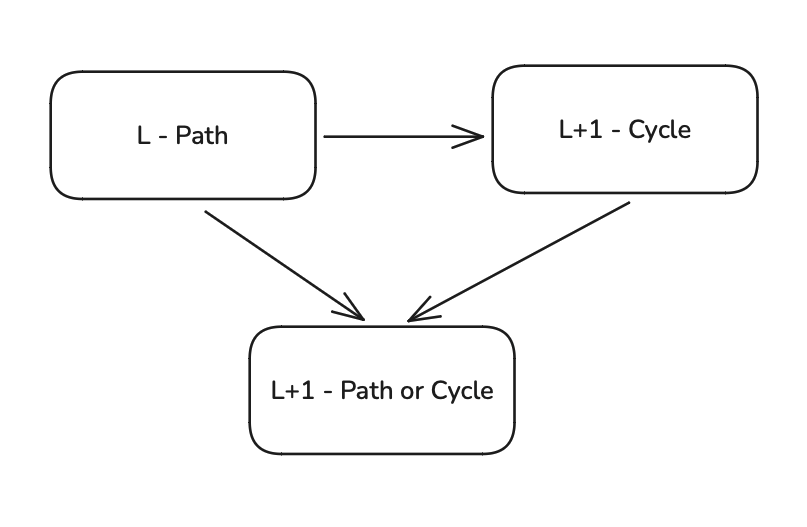
\includegraphics[width=\textwidth]{figuras/flowchart.png}
    \captionof{figure}{Algorithm flowchart}
}

%%%%%%%% Right Column (spans 6 of 12 columns) %%%%%%%%

% Algorithm Implementation
\posterbox[adjusted title = Algorithm Implementation]
          {name=algo, below=titlebox, column=7, span=6}{
    \begin{itemize}
        \item \textbf{Key Steps:}
        \begin{itemize}
            \item Start with initial object: empty path
            \item Incrementally extend the object
            \item When reach cycle of size $n-1$, there is a special case
        \end{itemize}
       
        \item \textbf{Complexity Analysis:}
        \begin{itemize}
            \item \textbf{Time Complexity:} $O(n^3)$
            \begin{itemize}
                \item Our object increment $O(n)$ times.
                \item Each increment takes $O(n^2)$ time.
            \end{itemize}
            Final time complexity: $O(n^3)$. It can't be improved because of the graph size.
            \item \textbf{Space Complexity:} $O(n^3)$
            
            For each graph, there are at most $n^2$ edges. We need to store all edges of all graphs.
        \end{itemize}
    \end{itemize}

    
}

% Visual Demo
\posterbox[adjusted title = Algorithm Visualization]
          {name=visual, below=algo, column=7, span=6}{
    \centering
    % \begin{figure}[H]
    %     \includegraphics[width=0.9\textwidth]{algorithm-steps}
    %     \caption{Key steps in finding a Rainbow Hamiltonian cycle}
    % \end{figure}
   
    \vspace{1em}
    \begin{minipage}{0.7\textwidth}
        \textbf{Animation Steps:}
        \begin{enumerate}
            \item Initial path construction
            \item Path extension phase
            \item Cycle completion
            \item Final Hamiltonian cycle
        \end{enumerate}
    \end{minipage}
}

% Results and Conclusion
\posterbox[adjusted title = Results and Conclusion]
          {name=conclusion, below=visual, column=7, span=6}{
    \begin{itemize}
        \item \textbf{Implementation Results:}
        \begin{itemize}
            \item Successfully tested on graphs up to size 300
            \item Average runtime: $O(n^2.8)$ in practice
            \item 100\% success rate on valid inputs
        \end{itemize}
       
        \vspace{1em}
       
        \item \textbf{Conclusion:}
        \begin{itemize}
            \item First practical implementation of Rainbow Dirac's theorem
            \item Efficient algorithm for finding Rainbow Hamiltonian cycles
            \item Applications in network design and routing
        \end{itemize}
    \end{itemize}
}

% Footer (spans both columns)
\posterbox[footerbox]{name=footerbox, above=bottom, column=1, span=12}{
    \large
    Department of Computer Science --- University of São Paulo\par
    \vspace{4pt}
    \small\ttfamily
    \{your-email\}@usp.br\par
    \vspace{4pt}
    \footnotesize\rmfamily
    GitHub: \texttt{your-username}
}

\end{tcbposter}

\end{document}
